\chapter{Prototyping}\label{chp:prototyping}


%===================================================================================================%
\section{Introduction}
%===================================================================================================%

After evaluating different requirements and therefore task/environment characteristics in chapter \ref{chp:suitabilityAssessment} and chapter \ref{chp:viabilityAssessment}, test cases and prototypes to 

%===================================================================================================%
\section{Containerized Application}
%===================================================================================================%


For the non-serverless approach, containers running the prototype are deployed on a Kubernetes Cluster on IBM Cloud. To adequately compare the prices of both solutions, a cluster type has to be chosen that is theoretically capable of the same compute power a serverless approach can deliver. The following system model is based on approximations and assumptions since non-serverless and serverless compute power is not possible to directly compare.

To illustrate, the smallest serverless instance type at AWS consists of function invocations with 128mb of RAM\footnote{\url{https://aws.amazon.com/lambda/pricing/}}. For the aforementioned scenario of $10,000$ messages per second, that would mean that at least 1280GB RAM is available at any given second (\(10,000 * 0.128\)) because this would be the allocated RAM when receiving $10.000$ messages at once. If the functions to process the messages run for more than one second the allocated RAM would drastically increase. For instance, if each function runs for three seconds, the allocated memory would increase threefold since every second 1280GB of RAM will be added to the overall allocation pool.\\
Under the hypothesis, that the simple unit conversion processing task outlined in chapter \ref{ssec:scaling} (page \pageref{ssec:scaling}) will not use 128MB memory per conversion, it is not necessary for the environment design to model a non-serverless environment that has the full 1280GB memory available but should be close to it. 

IBM Cloud provides users with three classes of cluster configurations:\footnote{\url{https://console.bluemix.net/pricing/configure/iaas/containers-kubernetes}}

\begin{minipage}{\textwidth}
    \begin{enumerate}[nolistsep]
        \item \textbf{Lite}\\
            Free of cost. Consists of one worker node.
        \item \textbf{Shared}\\
            Worker nodes that are shared with other IBM customers.
        \item \textbf{Dedicated}\\
            Dedicated worker nodes that ensure complete isolation of the physical ressources.
    \end{enumerate}
\end{minipage}

The available Kubernetes cluster options are as follows:\footnote{\url{https://console.bluemix.net/pricing/configure/iaas/containers-kubernetes}}

\begin{minipage}{\textwidth}
        \begin{tabular}{ | c | c | } 
            \hline
             \textbf{Plan} & 
             \textbf{Features}\\
             \hline \hline
             Lite & 
             2 CPUs, 4 GB RAM, 1 Worker Node\\
             \hline 
             2x4 - Shared & 
             2 CPUs, 4 GB RAM, 100GB HDD\\
             \hline 
             4x16 - Shared & 
             4 CPUs, 16 GB RAM, 100GB HDD\\
             \hline 
             16x64 - Shared & 
             16 CPUs, 64 GB RAM, 100GB HDD\\
             \hline  
             32x128 - Shared & 
             32 CPUs, 128 GB RAM, 100GB HDD\\
             \hline  
             56x242 - Shared & 
             56 CPUs, 242 GB RAM, 100GB HDD\\
             \hline 
             2x4 - Dedicated & 
             2 CPUs, 4 GB RAM, 100GB HDD\\
             \hline 
             4x16 - Dedicated & 
             4 CPUs, 16 GB RAM, 100GB HDD\\
             \hline 
             16x64 - Dedicated & 
             16 CPUs, 64 GB RAM, 100GB HDD\\
             \hline  
             32x128 - Dedicated & 
             32 CPUs, 128 GB RAM, 100GB HDD\\
             \hline  
             56x242 - Dedicated & 
             56 CPUs, 242 GB RAM, 100GB HDD\\
             \hline 
        \end{tabular}
        \centering
\end{minipage}


\begin{figure}[ht]
    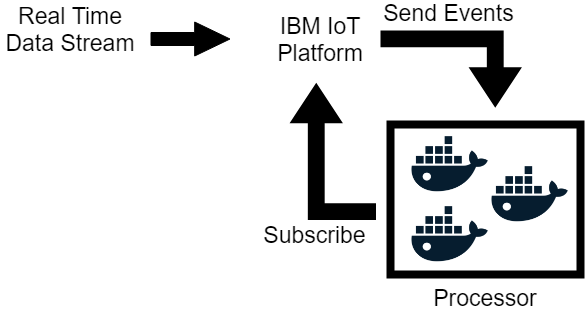
\includegraphics[width=0.6\linewidth]{images/streaming/containerArch.png}\centering
    \caption
    [IBM IoTP Managed Container Architecture]
    {IBM IoTP Managed Container Architecture}
    \label{fig:iotpManagedContainer}
\end{figure}

\begin{figure}[ht]
    \begin{lstlisting}[language=js,firstnumber=1]
    'use strict'
        
    const celsiusToFahrenheit = (eventType, format, payloadRaw) => {
      const payload = JSON.parse(payloadRaw)
      const fahrenheitTemp = (payload.temp / (9/5) + 32)
      console.log(fahrenheitTemp)
    }
        
    app.connect()
        
    app.on('connect', () => {
        app.subscribeToDeviceEvents()
    })
        
    app.on('deviceEvent', celsiusToFahrenheit)
    \end{lstlisting}\centering
    \caption{Code: Non-Serverless Processor}
    \label{code:nslProcessor2}
\end{figure}


%===================================================================================================%
\section{Serverless}
%=======================================================

\begin{figure}[ht]
    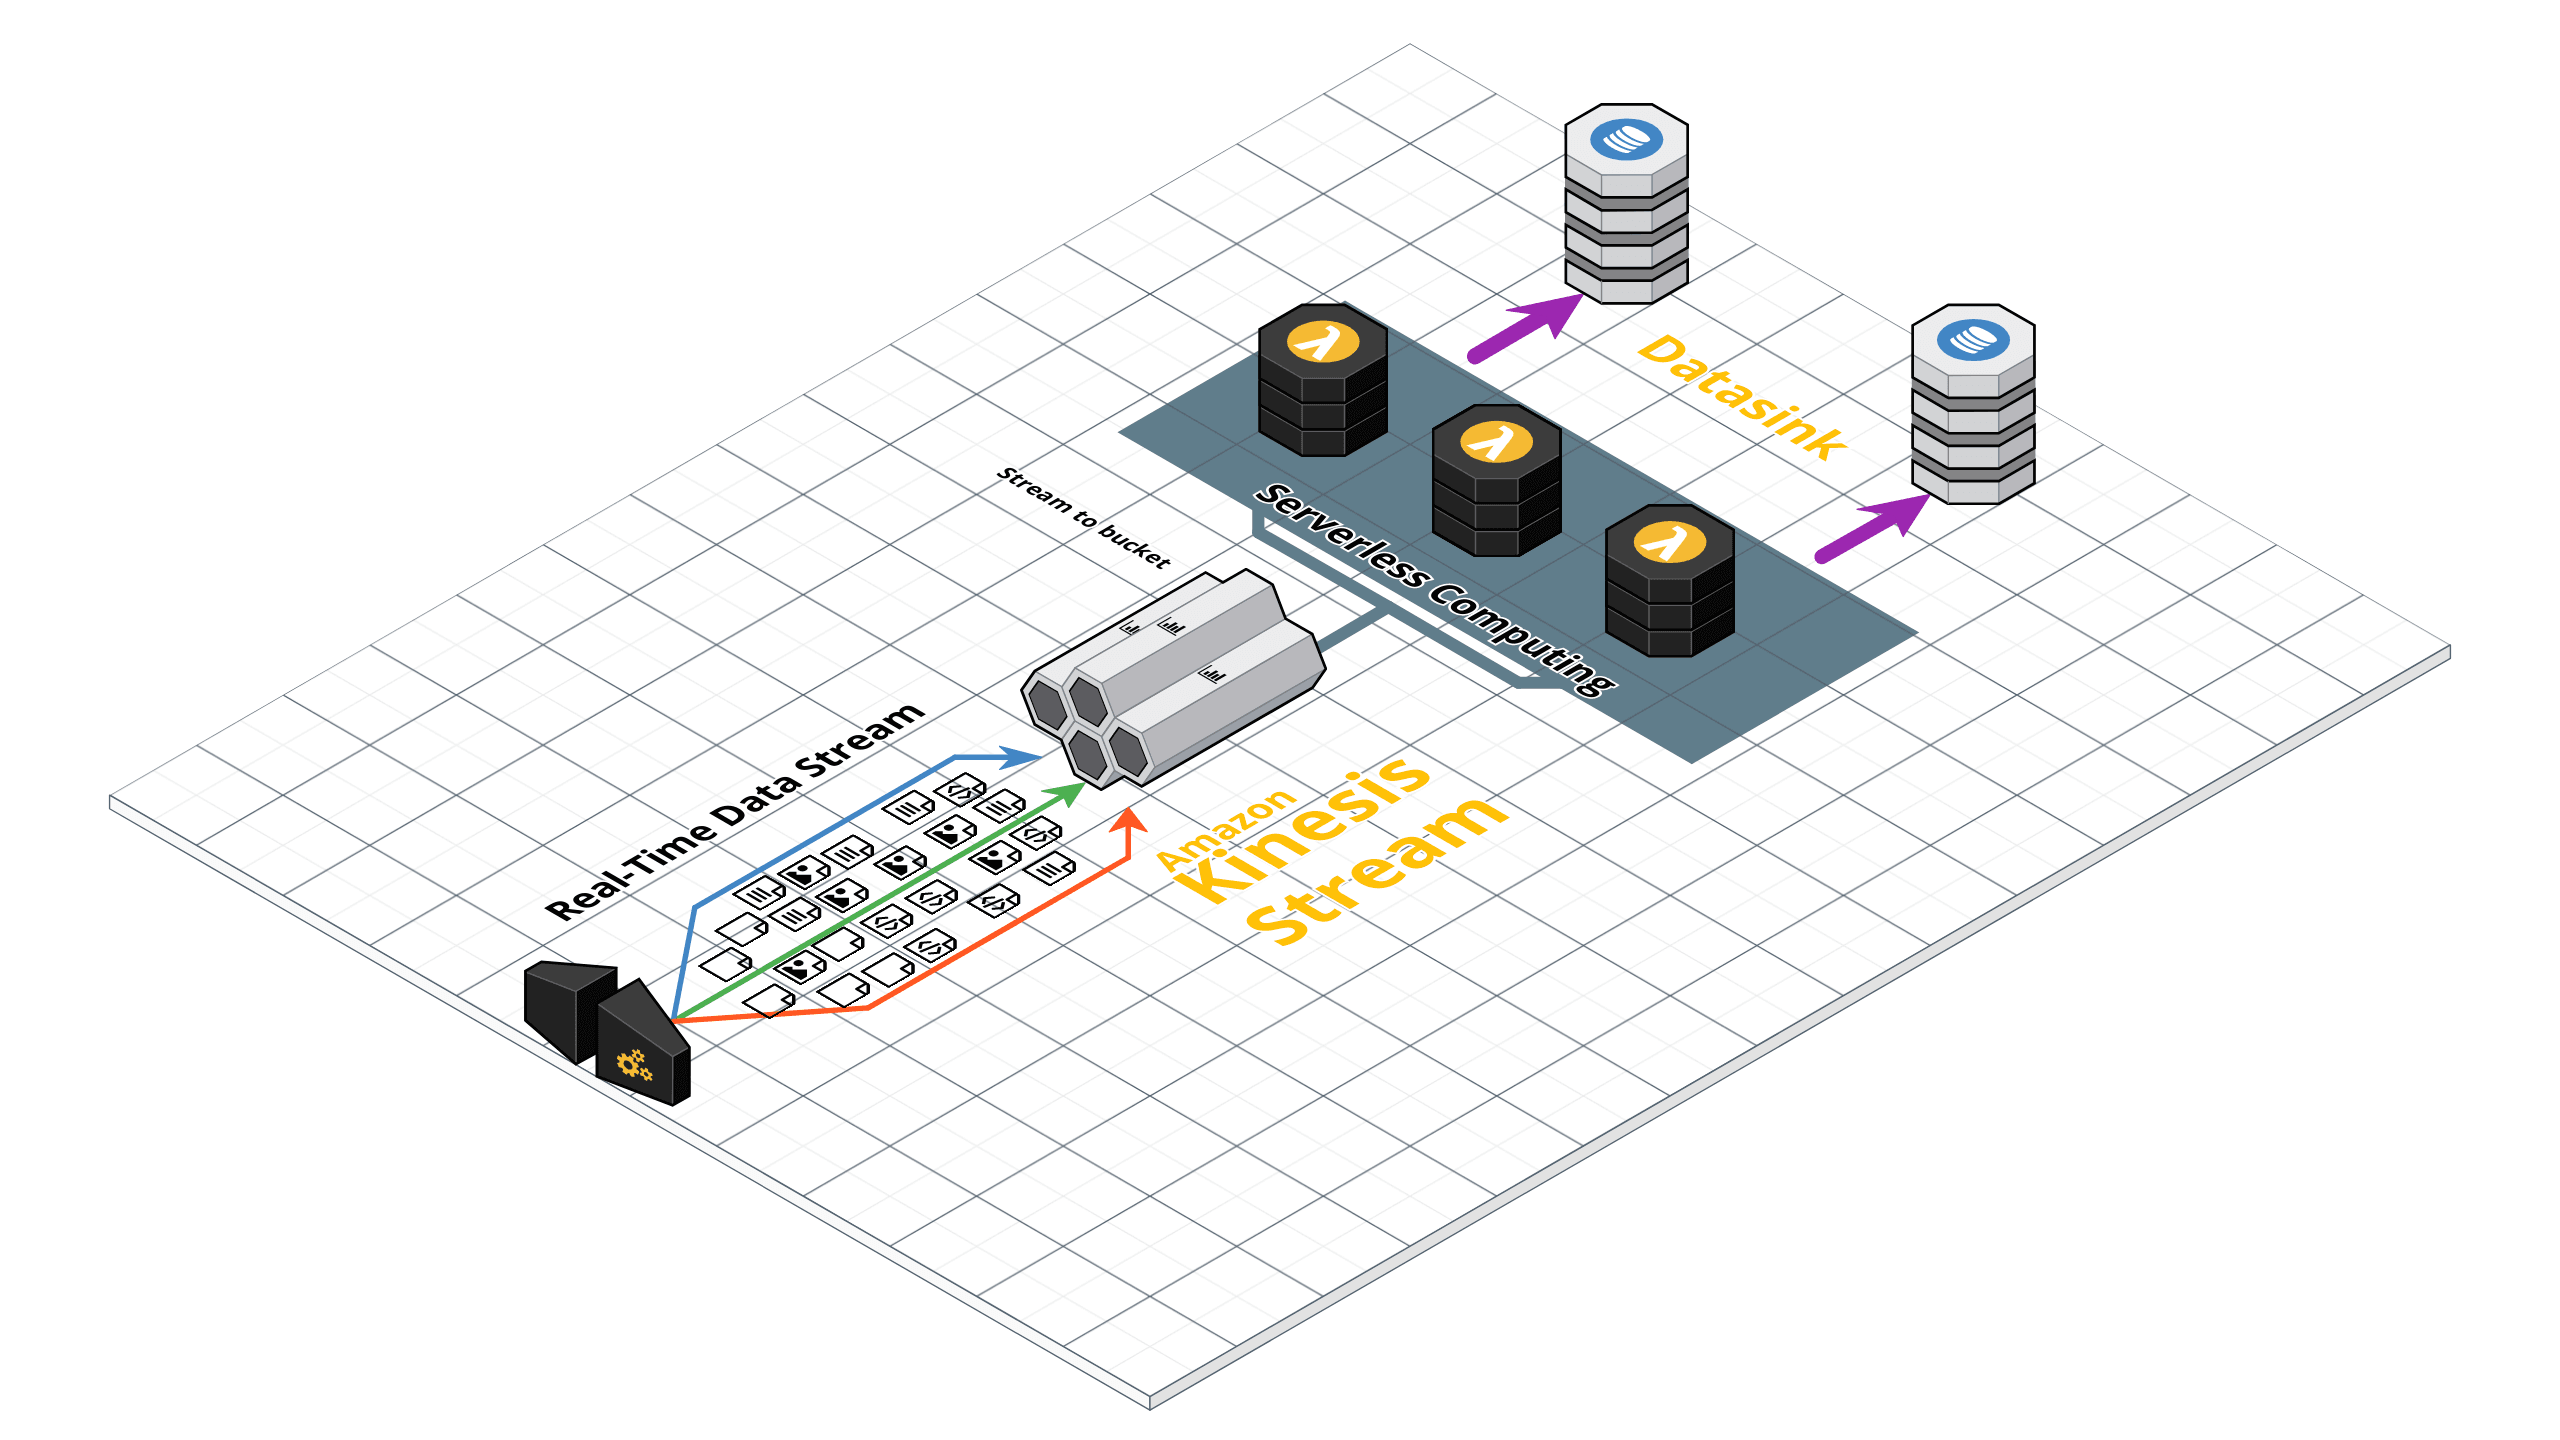
\includegraphics[width=\linewidth]{images/streaming/streamingaws.png}\centering
    \caption
    [AWS Stream Processing Architecture]
    {AWS Stream Processing Architecture}
    \label{fig:awsStreamingArchitecture}
\end{figure}

\begin{figure}[ht]
    \begin{lstlisting}[language=js,firstnumber=1]
    'use strict'

    const celsiusToFahrenheit = (eventType, format, payloadRaw) => {
      const payload = JSON.parse(payloadRaw)
      const fahrenheitTemp = (payload.temp / (9/5) + 32)
      return fahrenheitTemp
    }
        
    exports.handler = (event, context, callback) => {
        /* Process the list of records and transform them */
        const output = event.records.map((record) => ({
            /* This transformation is the "identity" transformation, the data is left intact */
            recordId: celsiusToFahrenheit(record.recordId),
            result: 'Ok',
            data: record.data,
        }))
        console.log(`Processing completed.  Successful records \${output.length}.`)
        callback(null, { records: output })
    };
    \end{lstlisting}\centering
    \caption{Code: Serverless Processor}
    \label{code:slProcessor}
\end{figure}

Chapter: \ref{chp:operationalization}








%===================================================================================================%
\section{Summary}
%===================================================================================================%

well, wex got two prototypes.